
\section{Introduction}

The purpose of this document is to describe the specification and design activities for the OpenETCS project. The activities for safety, verification and validation are not in the scope of this document and will be described in WP4's documents.

To deal with a safety process, the specification and design activities shall follow the requirements of EN 50126, EN 50128 and EN 50129 and reflect usual activities for the development of railway critical systems (see D2.1  and D2.2).
This description is linked to the set of requirements defined for the OpenETCS project in D2.6.

\subsection{Motivation}

This document describes the process to  be applied  during the OpenETCS project to achieve the main goals of the OpenETCS project:

\paragraph{A semi-formal reference specification for the ETCS requirements and architecture, completed by strictly formal  models of sub-parts}
The first goal of the project is to propose a semi-formal specification of the ETCS on-board functionalities according to  UNISIG SUBSET-026, baseline 3.

The purpose of this model is:
\begin{itemize}
\item to enhance the understanding of the subset;
\item to be able to animate the model for testing and analysing purpose at system level;
\item to provide information on the completeness and soundness of the SUBSET-026;
\item to be used as a reference semi-formal specification for the implementation of an on-board unit
(by the OpenETCS project team and by industrial actors);
\end{itemize}

The output is a model, at least semi-formal, understandable by many formal approaches (SCADE,
Simulink, B tools, OpenETCS tool chain…) that can be given to all railway actors, and
if possible associated to SRS documents in the ERA database.

Thus, strictly formal models can be designed from this semi-formal model which allows for formal proofs of sub-parts of SUBSET-026. This will allow improving the understanding of the system, and will provide elements for verification and validation using formal proof.

The final goal is that industrial actors work with this model instead of the
natural language specification.
The objective is to cover as much as possible of the  functionality of the on-board unit described in SUBSET-026 and to show the capabilities of analyses of a complex system using formal approaches.

\paragraph{Define the safety case concept for the full model and apply it on a subset of the on-board unit}
The safety strategy and the safety case concept required for the full validation of the product, compliant to the CENELEC standards shall be taken into account in all steps of the specification and design process. This will allow industrial actors to reuse the models and processes to develop certifiable products.

In particular the definition of the process shall take into account specification as well as verification and validation of the safety properties on the models. The outputs of WP4 (safety plan, safety case concept, verification plan and validation plan) will complete the description of the safety process.


\paragraph{Provide a tool chain and process/methodologies for developing
an on-board software that can fulfil the CENELEC requirements for SIL4 software}

The design process of the system and the associated tools of the tool chain, shall be suitable to provide a certifiable product. For this purpose all steps of the process and the choice of the methods and tools shall be justified to ensure a safe approach to build an ETCS system.

The full safety process required to make OpenETCS \emph{certifiable} according to CENELEC 50126, 50128 and 50129 shall be described in detail. The safety process will detail precisely which activities are required, why they are required, and the choices that are made to claim that a safe design process is guaranteed.

The use of formal methods, supported by tools, is highly recommended in this safety process for specification, design, verification and validation of the certifiable product.

The tool chain should include model editors, code generators, verification tools (including formal provers), validation tools (including test generators, simulators,..), document generation, version management, maintenance facilities, \dots

\paragraph{Provide an executable software package generated from the specification of on-board ETCS}

An executable software of the specification shall be provided, as well as a non vital implementation of the on-board unit for laboratory test, simulation and as reference.

The output is the result of a functional implementation for the ETCS requirements and architecture which can be used by the industrial as reference.

\todo{ Does this executable take into account real-time constraints ? API ? from which model it is derived ? }
\todo{at which level of the V-cycle ? system  ? software ?}

Besides this executable software, the tool chain can be used to  generate certifiable executable software from the formal model of sub-parts of the on-board unit.


\subsection{Contents of this Document}

As the Quality Plan D1.3 focuses on means to apply during the OpenETCS project (for example open source approaches or Scrum organization) the aim of this document is to define the main steps which are necessary within the OpenETCS project to produce a certifiable system according to the CENELEC standards.
Safety, verification and validation activities are described in the outputs of WP4.

\todo{Give the references of WP4 deliverables}

The first part of this document focuses on the description of the mandatory steps of a life-cycle to design a critical system according to the CENELEC standards, as described in figure~\ref{fig:OETCSProcess}.

\begin{figure}[h]
  \centering
  \fbox{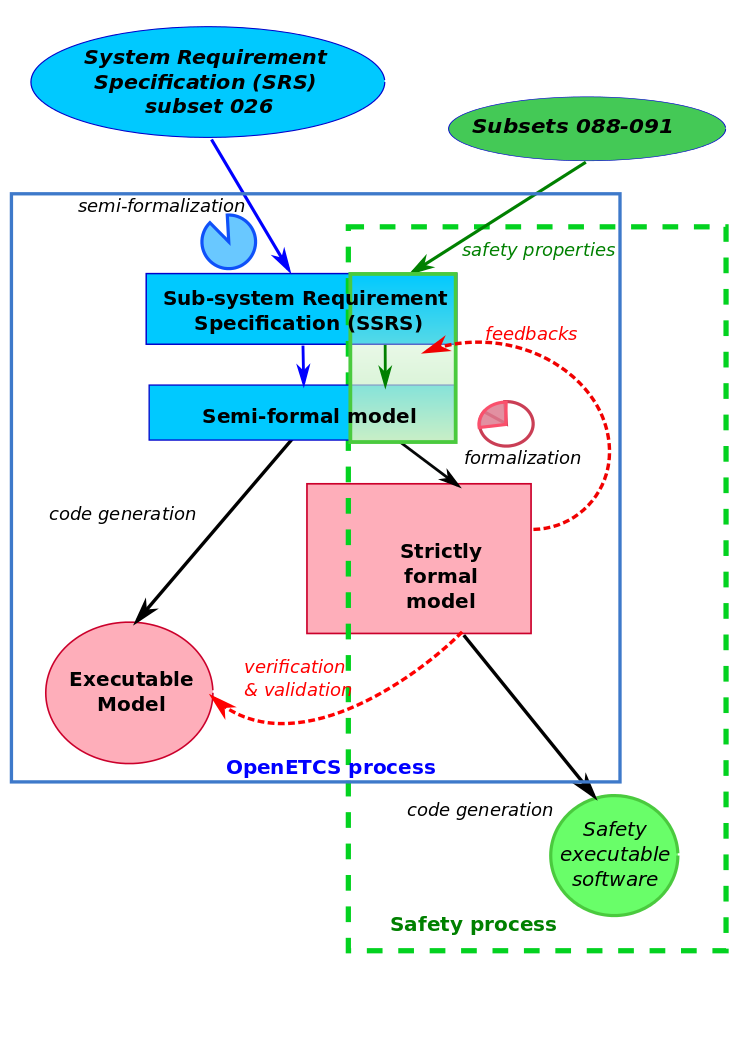
\includegraphics[width=4in]{OETCSProcess.png}}
  \caption{OpenETCS process}
  \label{fig:OETCSProcess}
\end{figure}


The proposed process for the OpenETCS project shall describe:
\begin{itemize}
\item how to design a semi-formal model of the on-board unit system from the SRS SUBSET-026 ;
\item how to design some subsets of the SRS SUBSET-026 within a safety process;
\item how to produce a running model of the application software of the on-board unit.
\end{itemize}

For the 2 first objectives, the semi-formal  model  shall take into account the safety constraints to apply to the design of a critical railway system.

The second part of this document describes the system to design during the OpenETCS project, as well as the scope of the safety activities on this system.

%%%%%%%%%%%%%%%%%%%%%%%%%%%%%%%%%%%%%%%%%%%%%%%%%%%%%%%%%%%%%%%

\section{Reference Documents}
\begin{itemize}
\item CENELEC EN 50126-1 --- 01/2000 --- \emph{Railways applications –- The specification and
demonstration of Reliability, Availability, Maintainability and Safety (RAMS) –- Part 1:
Basic requirements and generic process}
\item CENELEC EN 50128 --- 10/2011 --- \emph{Railway applications -- Communication, signalling and
processing systems -- Software for railway control and protection systems}
\item CENELEC EN 50129 --- 05/2003 --- \emph{Railway applications –- Communication, signalling and
processing systems –- Safety related electronic systems for signalling}
\item FPP --- \emph{Project Outline Full Project Proposal Annex OpenETCS} -- v2.2
\item SUBSET-026 3.3.0 --- \emph{System Requirement Specification}
\item SUBSET-076-x 2.3.y --- Test related ERTMS documentation
\item SUBSET-088 2.3.0 --- \emph{ETCS Application Levels 1 \& 2 - Safety Analysis}
\item SUBSET-091 3.2.0 --- \emph{Safety Requirements for the Technical Interoperability
of ETCS in Levels 1 \& 2}
\item CCS TSI --- \emph{ CCS TSI for HS and CR transeuropean rail has been adopted by a Commission Decision 2012/88/EU on the 25th January 2012}
\item D1.3 -- Project Quality Assurance Plan
\item D2.1 -- Report on existing methodologies 
\item D2.2 -- Report on CENELEC standards
\item D2.6 -- Requirements for OpenETCS
\end{itemize}

%%%%%%%%%%%%%%%%%%%%%%%%%%%%%%%%%%%%%%%%%%%%%%%%%%%%%%%%%%%%%%%

\section{Conventions}
The requirements are prefixed by “R-zz-x-y”, and are written in a roman typeface, where ``R''
stands for ``Requirement'', ``zz'' identifies the source document,``x''
is the version number and``y'' is the identifier of the requirement. All the text
written in italics is not a requirement: it may be a note, an open issue, an
explanation of the requirements, or an example.

The placeholder “\todo{xxx}” is used to indicate an unfinished  paragraph or section which is
to be defined or confirmed.

%%%%%%%%%%%%%%%%%%%%%%%%%%%%%%%%%%%%%%%%%%%%%%%%%%%%%%%%%%%%%%%

\section{Glossary}
\begin{description}
\item[API] Application Programming Interface
\item[FME(C)A] Failure Mode Effect (and Criticity) Analysis
\item[FIS] Functional Interface Specification
\item[HW] Hardware
\item[I/O] Input/Output
\item[OBU] On-Board Unit
\item[PHA] Preliminary Hazard Analysis
\item[QA] Quality Analysis
\item[RBC] Radio Block Center
\item[RTM] RunTime Model
\item[SIL] Safety Integrity Level
\item[SRS] System Requirement Specification
\item[SSHA] Sub-System Hazard Analysis
\item[SSRS] Sub-System Requirement Specification
\item[SW] Software
\item[THR] Tolerable Hazard Rate
\item[V\&V] Verification \& Validation
\end{description}
